\chapter{Descripción de Security Onion}
    \begin{section}{Security Onion como sistema de gestión de eventos}
    \begin{figure}[H]
        \centering
        
\includegraphics[width=0.7\textwidth]{./descripcion_sonion_imagenes/figura_15_logo_sonion.png}
        \caption{logo de Security Onion\cite{sonion}}
        \label{fig:logo_sonion}
    \end{figure}
        La elección de Security Onion (versión 16.04) como plataforma se justificó en su naturaleza de código abierto y por sus características destacables respecto de otras soluciones libres, como el soporte de una activa comunidad, el desarrollo continuo de mejoras, actualizaciones y correcciones, su capacidad polimórfica y funcional de actuar como IDS, plataforma SIEM o cluster de almacenamiento. Esto permitió desarrollar distintas arquitecturas de una manera fácil y asistida para el despliegue y la consiguiente optimización de los recursos de hardware y de red. \par
        Otras de las propiedades destacables es la capacidad de integración directa con un conjunto casi universal de los sistemas IDS disponibles, tanto libres como propietarios. Security Onion también incluye un paquete de configuraciones iniciales predefinidas para la infraestructura inicial del sistema, tales como el almacenamiento, normalización y gestión de logs, sistemas IDS y de gestión de usuarios, entre otros. \par
    \end{section}
    \begin{section}{Arquitectura del sistema de gestión de eventos}
    \end{section}
    \begin{subsection}{Arquitectura de alto nivel}
    \begin{figure}[H]
        \centering
        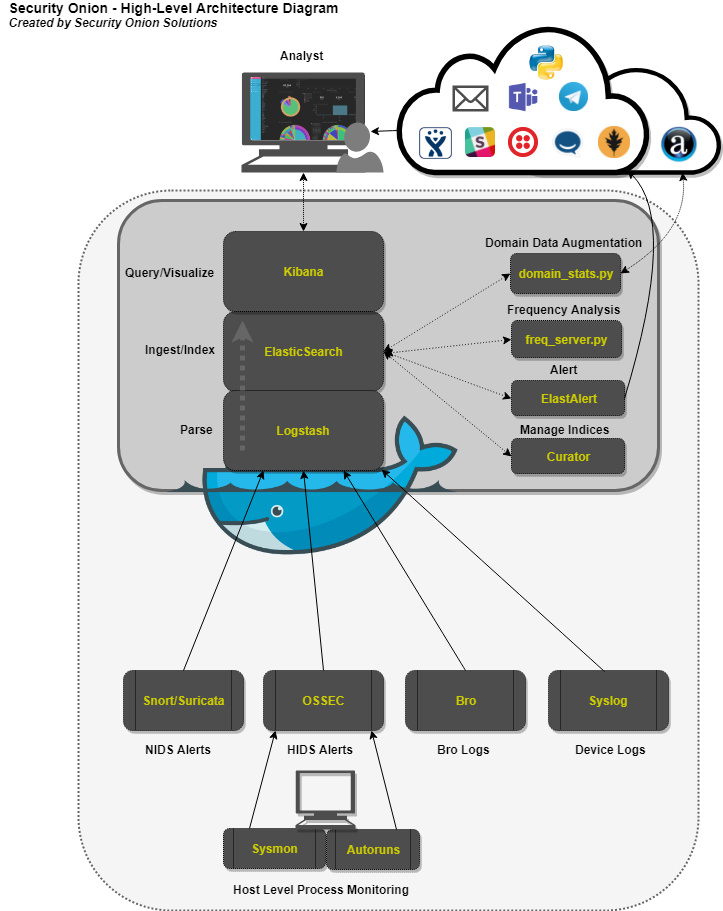
\includegraphics[width=0.7\textwidth]{./descripcion_sonion_imagenes/figura_16_arq_alto_nivel_sonion.png}
        \caption{Security Onion\cite{sonion}: Arquitectura de alto nivel}
        \label{fig:arq_top_sonion}
    \end{figure}
    En la Figura \ref{fig:arq_top_sonion} se observa la distribución de Security Onion y el flujo de datos entre sus componentes principales (la pila Elastic) y secundarios (Curator \cite{curator}, ElastAlert\cite{elasalert}, freqServer\cite{freqserver} y domainStats\cite{domainstat}). Se puede apreciar la conexión con los sistemas de detección IDS como Bro\cite{zeek}, Snort\cite{snort}, Suricata\cite{suricata}, Syslog, etc. Se distinguen también los enlaces con los puntos de administración de los analistas del CSIRT y con los servicios web externos para el envío y recepción de alertas, notificaciones, análisis de tráfico, entre otros. Un punto a destacar es que la pila Elastic se encuentra desplegada en contenedores Docker\cite{docker}. 
    \end{subsection}
    \pagebreak
    \begin{subsubsection}{Tipo de Nodos}
        \begin{itemize}
          \item Nodo Master: este nodo ejecuta su propia copia de la base de datos Elasticsearch, con la que gestiona las búsquedas a través del cluster y estructura a otros nodos en el momento de su despliegue. Lo anterior implica que puede realizar las configuraciones necesarias para los nodos de los tipos “densos” y los de almacenamiento, pero no los de sensores o Forward, por carecer estos últimos de una pila Elastic. Este nodo permite a un analista conectarse mediante un enlace de administración para realizar consultas de los datos.
          \begin{itemize}
              \item  Este nodo contiene los siguientes componentes:
              \begin{itemize}
                  \item Elasticsearch \cite{elastic}
                  \item Logstash \cite{elastic}
                  \item Kibana \cite{elastic}
                  \item Curator \cite{curator}
                  \item ElastAlert \cite{elasalert}
                  \item Redis \cite{redis}
                  \item Wazuh \cite{wazuh} / OSSEC \cite{ossec}
                  \item Sguild \cite{sguil}
              \end{itemize}
          \end{itemize}
          Elasticsearch \cite{elastic}, Kibana \cite{elastic} y Logstash \cite{elastic} son componentes de la pila Elastic, que se tratarán en la siguiente sección junto a ElastAlert \cite{elasalert}. El objetivo de Curator \cite{curator} y Redis \cite{redis} es administrar y optimizar las bases de datos de los nodos de almacenamiento; Wazuh \cite{wazuh} es un IDS y Security Onion lo utiliza para el monitoreo de sí mismo, configurando un sistema HIDS ad hoc, aunque es posible desplegarlo en otros nodos o puntos de interés. Sguild \cite{sguil} permite consultar eventos de una base de datos MySQL desde dentro de Security Onion y muestra los resultados en una GUI. Además, actúa como intermediario de otros componentes secundarios como Squert \cite{squert}, del que detallaremos sus funciones y comportamiento en una sección posterior. 
          \item Nodos Forward: este nodo cumple la función de procesar el tráfico y reenviar los resultados al nodo master. Los logs generados por Snort / Suricata y Bro son enviados mediante syslog a Logstash en el nodo Master, utilizando un túnel ssh, donde finalmente son guardados en la base de datos Elasticsearch, donde pueden ser reenviados a los nodos de almacenamiento. Los logs pueden ser consultados a través de una búsqueda en el cluster.
            \begin{itemize}
               \item Los componentes de un nodo Forward son:
               \begin{itemize}
                   \item Zeek \cite{zeek} (sucesor de Bro)
                   \item Snort \cite{snort} / Suricata \cite{suricata}
                   \item Netsniff-ng \cite{netsniff-ng}
                   \item Wazuh \cite{wazuh} / OSSEC \cite{ossec}
                   \item Syslog-ng \cite{syslog-ng}
               \end{itemize}
            \end{itemize}
            Zeek, Snort / Suricata y Netsniff-ng son procesadores de tráfico (IDS), donde Snort y Suricata serán tratados en una sección posterior. Syslog-ng es utilizado para recolectar logs de los IDS y enviarlos al Logstash del master, donde serán procesados y tratados antes de ser escritos en Elasticsearch.
            \item Nodos Pesados (Heavy Nodes): Es un nodo híbrido entre el nodo Forward y el nodo Master, que incluye todos los componentes del nodo Forward, además de una instancia completa de la pila Elastic. Los nodos pesados envían los resultados de las consultas de su instancia local de Elasticsearch a las solicitudes realizadas por el nodo master mediante un túnel de autossh.
            \begin{itemize}
                \item Los componentes de este nodo son:
                \begin{itemize}
                    \item Elasticsearch
                    \item Logstash
                    \item Curator
                    \item Zeek
                    \item Snort / Suricata
                    \item Netsniff-ng
                    \item Wazuh / OSSEC
                    \item Syslog-ng (envía los logs a la instancia local de Logstash)
                \end{itemize}
            \end{itemize}
            \item Nodos de almacenamiento (Storage Node): su objetivo es extender las capacidades de almacenamiento y procesamiento del nodo Master. Estos nodos despliegan una instancia local de la pila Elastic. De manera análoga a los nodos pesados, cuando se realiza una consulta por parte de la instancia Elasticsearch del nodo Master, esta es procesada por la instancia local del nodo de almacenamiento y devuelta por un túnel autossh.
            \begin{itemize}
                \item Los componentes del nodo de almacenamiento son:
                \begin{itemize}
                    \item Elasticsearch
                    \item Logstash
                    \item Curator
                    \item Wazuh / OSSEC
                \end{itemize}
            \end{itemize}
        \end{itemize}
    \end{subsubsection}
    \pagebreak
    \begin{subsubsection}{Tipos de Arquitectura}
    \label{tipos_de_arquitectura}
      La versatilidad de disponer de múltiples arquitecturas permite adaptar la plataforma a las necesidades de la organización en la que se implante. A continuación, se describen cada una de las opciones posibles:
    \begin{itemize}
         \item Arquitectura monolítica: Consiste en un único servidor que ejecuta simultáneamente los componentes centrales o propios de un nodo Master y los de un nodo sensor. Es un modo híbrido y concentrado que no se recomienda para enlaces de red de alto rendimiento por los elevados requerimientos de hardware necesarios. 
         Este tipo de arquitectura se recomienda para propósitos de pruebas en laboratorio y en entornos de baja demanda de tráfico de red.
        \begin{figure}[H]
            \centering
            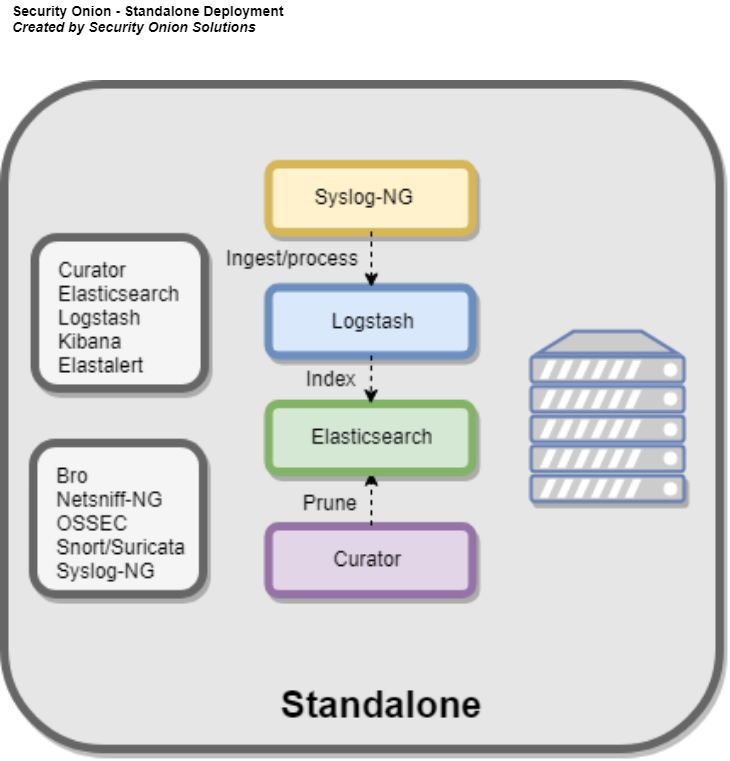
\includegraphics[width=0.7\textwidth]{./descripcion_sonion_imagenes/figura_17_arq_monolitica_sonion.png}
            \caption{Arquitectura monolítica de Security Onion\cite{sonion}}
            \label{fig:arq_monolitica_sonion}
        \end{figure}
        \FloatBarrier
        \pagebreak
        \item Arquitectura densamente distribuida: consiste en uno o más nodos pesados (Heavy Nodes) conectados a un nodo Master. Solo se recomienda en el caso de que no sea posible desplegar una arquitectura distribuida, ya que tiene las mismas deficiencias de rendimiento de la arquitectura monolítica y no es apropiado para entornos de producción y/o enlaces de red de alta velocidad.
        \begin{figure}[H]
            \centering
            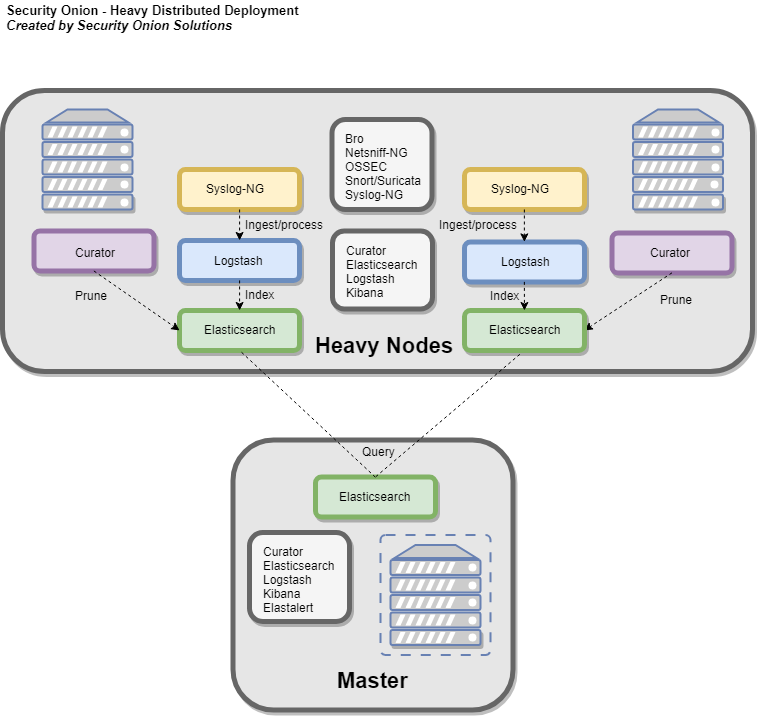
\includegraphics[width=0.7\textwidth]{./descripcion_sonion_imagenes/figura_18_arq_densa_sonion.png}
            \caption{Arquitectura densamente distribuida de Security Onion\cite{sonion}}
            \label{fig:arq_densa_sonion}
        \end{figure}
        \FloatBarrier
        \pagebreak
        \item Arquitectura Distribuida: consiste en un servidor Master, uno o más nodos Forward y uno o más nodos de almacenamiento (Storage Nodes). Es el tipo de despliegue recomendado en términos de eficiencia de requerimientos de hardware, balance de la carga y almacenamiento de datos y optimización general de los recursos disponibles en la organización. 
        \begin{figure}[H]
            \centering
            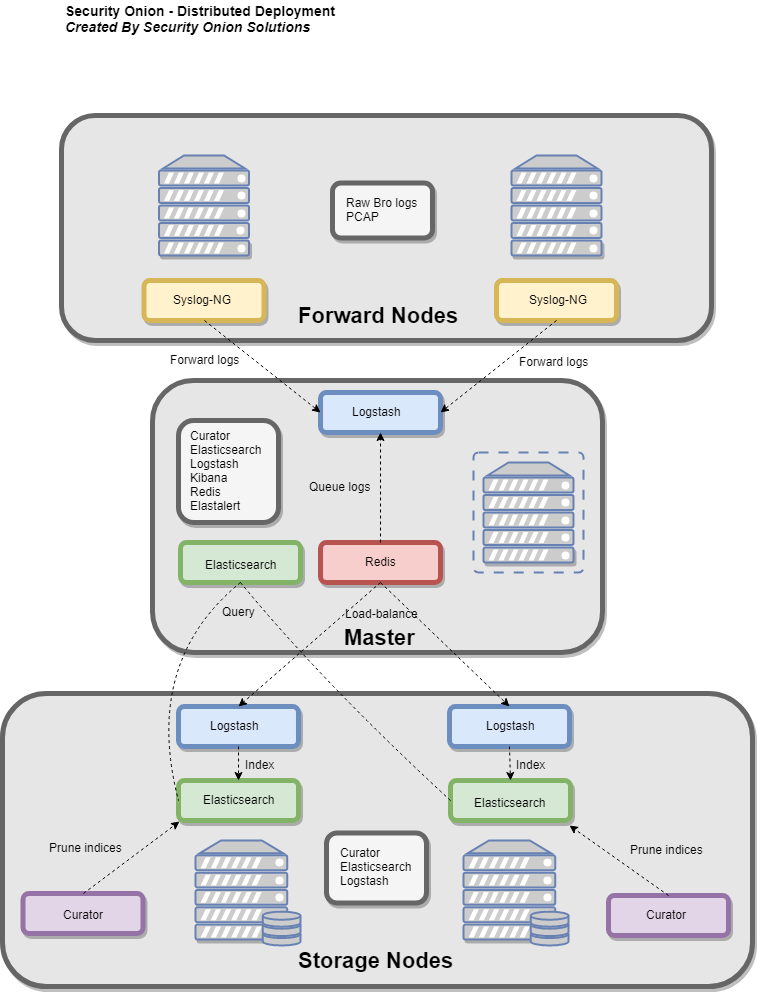
\includegraphics[width=0.7\textwidth]{./descripcion_sonion_imagenes/figura_19_arq_distribuida_sonion.png}
            \caption{Arquitectura distribuida de Security Onion\cite{sonion}}
            \label{fig:arq_distribuida_sonion}
        \end{figure}
     \end{itemize}
   \end{subsubsection}
   \pagebreak
  
   \begin{section}{Recibiendo, procesando y visualizando eventos: La pila Elastic}
   En la Figura \ref{fig:figura_20_conexion_comp_elastic} se observa, que luego de recolectar los datos provenientes de múltiples fuentes, es necesario normalizarlos y agregarlos a la base de datos; estas tareas son llevadas a cabo por los componentes de la pila Elastic (versión 6.8.0), en este caso Logstash y Elasticsearch, respectivamente. 

   \begin{figure}[H]
        \centering
        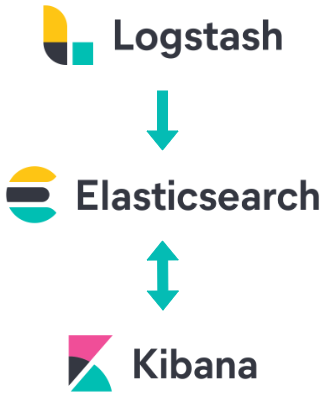
\includegraphics[width=0.45\textwidth]{./descripcion_sonion_imagenes/figura_20_conexion_comp_elastic.png}
        \caption{Conexión de componentes Elastic}
        \label{fig:figura_20_conexion_comp_elastic}
    \end{figure}
        
   \end{section}
   %\pagebreak
   \begin{subsection}{Logstash}
        Logstash es una tubería (en adelante “pipeline”) de procesamiento de datos del lado del servidor que ingesta datos de una multitud de fuentes, los transforma y luego los envía a su destino. Las fuentes de entrada admitidas por logstash son extremadamente amplias, como por ejemplo: syslog, STDIN, TCP, UDP, SNMP, IMAP, entre otras. Posteriormente, Logstash toma los datos sin estructura y los normaliza para crear conjunto ordenado mediante la identificación y conversión de la información a un formato común. Para realizar la tarea anterior, dispone de una gran variedad de filtros que facilitan el procesamiento general, independientemente de la fuente de datos. En este proyecto se utilizó el plugin grok (versión 4.0.4) \cite{grok} como filtro de las fuentes de información. Con los datos ya normalizados, es posible darles un formato específico para un destino en particular, ya que Logstash admite múltiples destinos para la etapa final del pipeline; desde una base de datos, archivos finales o servicios web. Security Onion, por defecto, almacena estos datos normalizados en un formato JSON en la misma pila Elastic, es decir la base de datos Elasticsearch.
   \end{subsection}
   
   \begin{subsection}{Elasticsearch}
        Elasticsearch es una base de datos del tipo NoSQL distribuida y orientada al almacenamiento de documentos. Los datos normalizados provenientes de Logstash son documentos almacenados en índices en Elasticsearch. Cada índice está compuesto por uno o más shards (fragmento), por lo tanto un shard es un subconjunto de documentos, siendo el elemento básico de Elasticsearch y el que permite la escalabilidad del mismo. Un shard es también una instancia de un “índice de Lucene \cite{lucene}", que indexa y almacena un documento en un segmento. Lucene es una librería desarrollada en Java (versión 8) para hacer búsquedas en una base de datos, constituyéndose en un motor de búsqueda que indexa y administra consultas en un conjunto de segmentos. La Figura \ref{fig:figura_21_arq_alm_elasticsearch} muestra la arquitectura de alto nivel del almacenamiento en Elasticsearch.
        
        \begin{figure}[H]
            \centering
            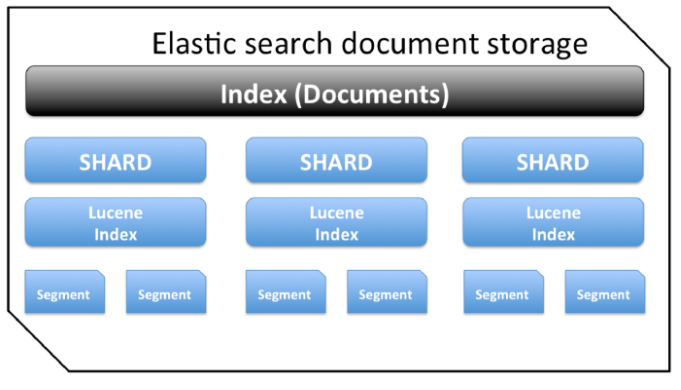
\includegraphics[width=0.7\textwidth]{./descripcion_sonion_imagenes/figura_21_arq_alm_elasticsearch.png}
            \caption{Arquitectura de almacenamiento en Elasticsearch}
            \label{fig:figura_21_arq_alm_elasticsearch}
        \end{figure}
    \end{subsection}
    %\pagebreak
    \begin{subsection}{Kibana}
     Todos los datos almacenados en Elasticsearch pueden ser visualizados por Kibana, una interfaz gráfica perteneciente a la pila Elastic. Kibana permite visualizar los datos en gráficos circulares, de barras, histogramas, etc e interactuar con ellos; también es posible realizar análisis de ubicación cuando se disponen de los metadatos correspondientes mediante el complemento Elastic Maps, realizar análisis de series temporales de una manera rápida y sencilla, dispone de herramientas de inteligencia artificial, que mediante aprendizaje no supervisado permite detectar anomalías y patrones mediante las proyecciones sobre los datos. \par
     Otra de sus características es  la posibilidad de realizar gráficos de correlación y entrecruzamiento, seleccionando campos de interés y filtros lógicos creados por el usuario. Es de destacar que para algunas de estas características es necesario la instalación de plugins complementarios y aunque en su inmensa mayoría son gratuitos, algunos pueden ser pagos ya que utilizan servicios web de la nube de los desarrolladores. 
     \begin{figure}[H]
        \centering
        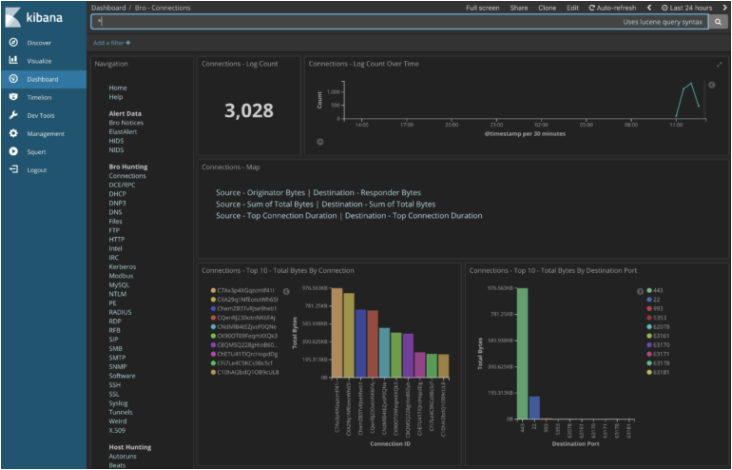
\includegraphics[width=1\textwidth]{./descripcion_sonion_imagenes/figura_22_capt_kibana.png}
        \caption{Captura de pantalla de Kibana\cite{elastic}}
        \label{fig:captura_kibana}
        \end{figure}
   \end{subsection}
   \begin{section}{Elastic, ElastAlert, TheHive y Cortex}
        Security Onion incluye la pila Elastic, cuyos componentes son Logstash quien se encarga de recibir, procesar, normalizar y agregar los datos resultantes a la base de datos  Elasticsearch y Kibana que permite visualizar estos datos. El proceso comienza cuando Logstash recibe los datos sin procesar provenientes de múltiples fuentes, son normalizados por este componente y enviados a Elasticsearch para su almacenamiento. Kibana permite consultar la base de datos mediante una interfaz gráfica de usuario y utilizar esa información para propósitos de análisis de amenazas. \par
        ElastAlert (versión 0.1.39) es un framework que permite identificar y alertar sobre eventos anómalos o patrones de interés sobre los datos de Elasticsearch. También provee múltiples mecanismos para enviar alertas mediante distintas plataformas externas, tales como Slack \cite{slack}, correo electrónico, JIRA \cite{jira}, Telegram \cite{telegram} y muchos más. Tanto ElastAlert como los componentes de la pila Elastic están desplegados sobre contenedores Docker (versión 19.03.12) \cite{docker}. \par
        Es destacable que, aunque Security Onion cubre gran parte de los requerimientos de un SIEM, no posee los elementos que permiten completar un sistema de manejo y respuesta a incidentes; por esta razón y luego de una investigación sobre las alternativas posibles, se incluyó a TheHive (versión 3.3.0) \cite{thehive} y Cortex (3.0.1-1) \cite{thehive} como complemento de Security Onion. TheHive permite la gestión de incidentes de manera detallada y la colaboración con otros CSIRT mediante el uso compartido de información sobre incidentes en tiempo real; mientras que Cortex hace posible la automatización de las respuestas y operaciones ante incidentes utilizando los datos enviados por TheHive. \par

   \end{section}
   \begin{section}{Correlación de eventos: ElastAlert}
     A pesar de que Kibana permite consultar los datos almacenados en Elasticsearch y presentarlos de diversas maneras que resultan en una gran utilidad, carece de la capacidad de generar alertas cuando los datos coinciden con algún patrón, especialmente cuando estos datos son escritos y consultados en tiempo real en la base de datos. Con este objetivo, la plataforma integra a ElastAlert, siendo un componente confiable, modular y simple de configurar. Su funcionamiento se basa en dos componentes principales: reglas y alertas. Las primeras son utilizadas para comparar con los datos resultantes de las consultas que se hacen en forma constante a Elasticsearch, esta comparación consiste en hallar patrones o firmas definidas en las reglas dentro de los datos obtenidos de la consulta; si el resultado de la búsqueda es positivo, una alerta es disparada para notificar el evento. \par
     Las alertas consisten en mensajes que permiten notificar a otro sistema con el objetivo de que este último realice una acción sobre las causas del evento que detectó la regla o bien informar a los analistas y/o responsables definidos. En cualquiera de los dos casos, las alertas pueden incluir toda la información recabada en un formato definido, tales como plantillas o cualquier arreglo configurado a tal fin. \par
     Según la naturaleza de los eventos a clasificar, las reglas cuentan con un conjunto común de paradigmas de monitoreo, estos permiten identificar y generar alertas aprovechando las características de las anomalías al mismo tiempo que optimizan los recursos del resto del CSIRT en términos de hardware y atención de los analistas. Algunos de estos paradigmas se basan en el comportamiento, tales como la frecuencia que consiste en generar una alerta cuando se detectan N cantidad de eventos en un intervalo definido, el cambio de tasas de ocurrencia por arriba o abajo de un límite establecido como normal para un determinado tipo de eventos, cuando en los datos se encuentran presente campos que han sido previamente establecidos como parte de una lista blanca, negra u algún campo cuyo valor coincida con otros tipos de filtros, entre otros. Es posible definir y configurar tantas reglas como alertas sean necesarias. \par

   \end{section}
   \pagebreak
   \begin{section}{El panel de control general: TheHive }
     Como se mencionó en las secciones anteriores, Security Onion requiere de otros elementos capaces de realizar la gestión integral de incidentes y sus respuestas, elementos que sean capaces de condensar y presentar información a los analistas del CSIRT encargados de monitorear y responder a las anomalías e incidentes detectados.  TheHive es la herramienta que se eligió para esta tarea ya que es una plataforma de respuesta a incidentes de seguridad gratuita y de código abierto, cumpliendo así con uno de los requerimientos no funcionales del proyecto, referido al tipo de licencia y accesibilidad al código. Otra de las razones para la elección de esta plataforma en particular ha sido su escalabilidad y su integración con MISP, lo que permite compartir información sobre las amenazas detectadas con otros CSIRT de organizaciones aliadas. Las tres capacidades centrales son la elaboración de casos, la respuesta a estos y la anteriormente mencionada colaboración con otros CSIRT.\par
     \begin{figure}[H]
        \centering
        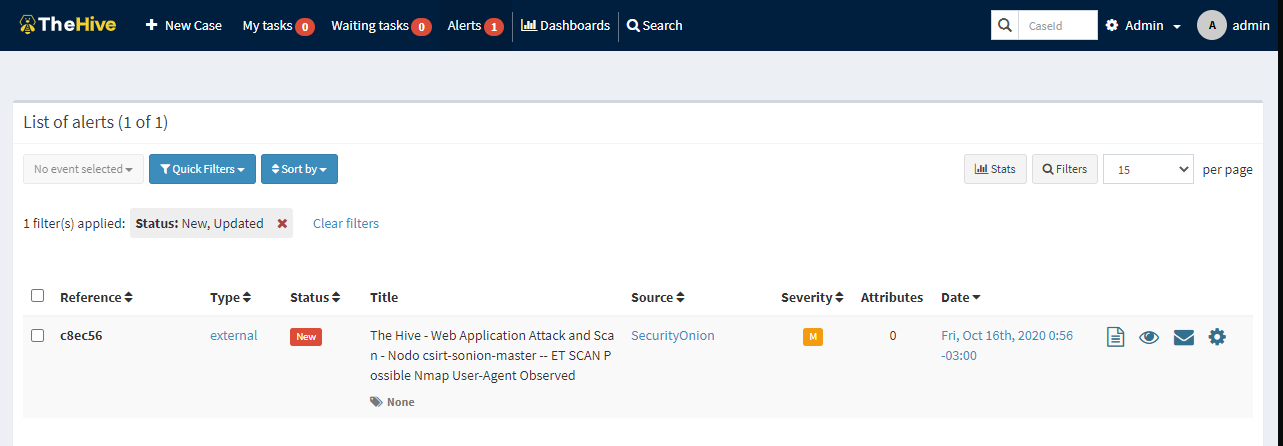
\includegraphics[width=1\textwidth]{./descripcion_sonion_imagenes/figura_23_alerta_panel_thehive.png}
        \caption{ Alertas recibidas en el panel de TheHive\cite{thehive}}
        \label{fig:alerta_panel_thehive}
     \end{figure}
        \FloatBarrier
        En cuanto a la elaboración de casos y tareas asociadas, estas se crean en base a las alertas recibidas \ref{fig:figura_21_arq_alm_elasticsearch}, donde el primer paso consiste en la creación de un caso para luego asociar este a una o varias de las alertas presentes utilizando la plantilla disponible \ref{fig:captura_kibana}, posteriormente es posible agregar tareas asociadas al caso, las cuales se pueden asignar a distintos analistas; a continuación es posible sumar métricas y campos personalizados, reducir el tiempo de búsqueda y recopilación de datos así como automatizar algunas tareas de recopilación de antecedentes en el manejo de incidentes mediante el uso del tablero, tal como se observa en la Figura \ref{fig:alerta_panel_thehive}. En el proceso de creación del caso, TheHive permite agregar cualquier otra información que se considere relevante, como etiquetas, archivos sospechosos de contener malware, etc a modo de evidencias.
        \begin{figure}[H]
        \centering
        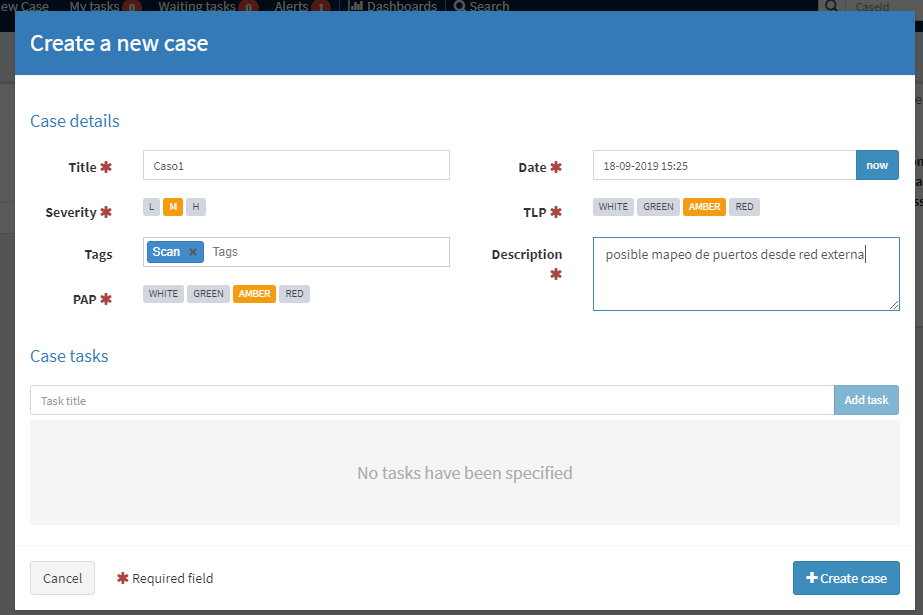
\includegraphics[width=1\textwidth]{./descripcion_sonion_imagenes/figura_24_plantilla_creacion_casos.png}
        \caption{Plantilla para la creación de nuevos casos}
        \label{fig:figura_24_plantilla_nuevos_casos}
     \end{figure}
     \FloatBarrier
     En las figuras \ref{fig:figura_24_plantilla_nuevos_casos} y \ref{fig:dashboard_dinamico} se observan la plantilla de creación de nuevos casos y el tablero que listan los casos existentes, respectivamente.
     \begin{figure}[H]
        \centering
        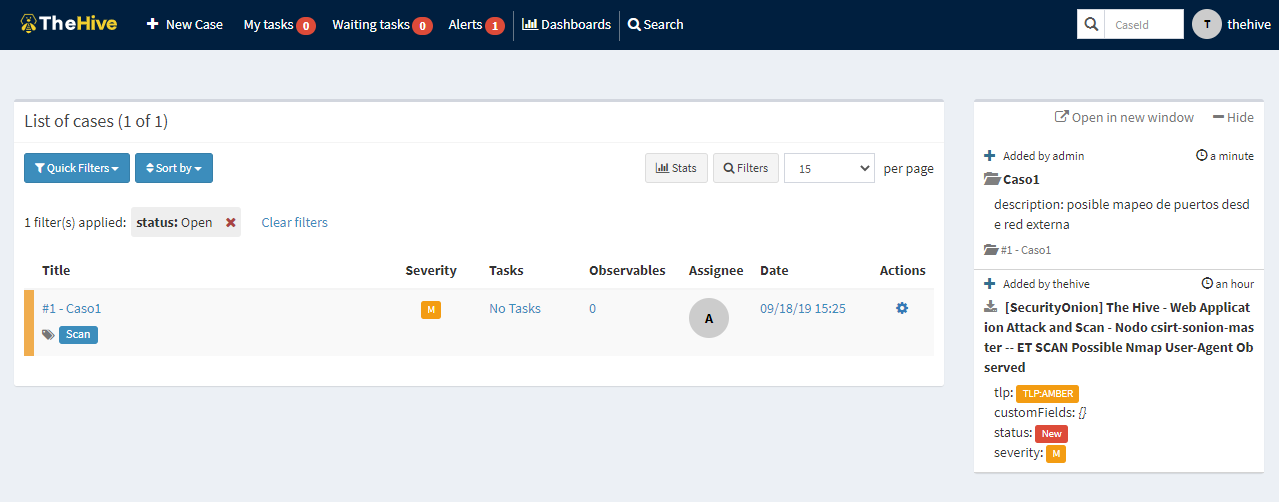
\includegraphics[width=1\textwidth]{./descripcion_sonion_imagenes/figura_25_dashboard_dinamico_thehive.png}
        \caption{Lista de casos de TheHive}
        \label{fig:dashboard_dinamico}
     \end{figure}
     \FloatBarrier
     Luego de la creación de un caso, es posible sumarle todos los “observables” que sean necesarios, donde los observables son todos aquellos campos que se pueden agregar de forma manual y que constituyen fuentes de información para analizar cada caso. Una vez configurado un caso, estos son examinados por scripts llamados “analyzers” que correlacionan y filtran los datos del caso contra los provistos por otras instancias MIPS u otras fuentes de información como la propia base de datos local, servicios de resolución DNS, plataformas como Shodan\cite{shodan}, VirusTotal\cite{virustotal}, Google Cloud Visión\cite{vision-AI}, entre muchas otras. Los observables también se pueden obtener por datos de las alertas recibidas, los cuales son previamente configurados en ElastAlert. Como se mencionó anteriormente ElastAlert realiza consultas a Elasticsearch y con los resultados busca patrones de interés para realizar una notificación, obtenida esta última extrae datos que se consideran de interés para ser enviados a The Hive. Un ejemplo de esto puede ser un número de IP, tipo de protocolo, fecha que se generó el log, puerto de origen y/o destino. La alerta que llega a The Hive contiene todos estos datos, considerados observables. \par
     En la Figura \ref{fig:caso_de_uso_gestion_usuario_conf_thehive} se puede observar los distintos casos de uso para la gestión de usuario que tiene TheHive. Se observa que el administrador puede gestionar usuarios, lo que implica crearlos, bloquearlos o generar API KEYs para ellos. También es posible crear o modificar plantillas de casos y reportes, crear nuevos casos y métricas para estos. Así mismo, existe la posibilidad de  crear Observables, alertas y gestionar estas últimas: TheHive permite ver las alertas recibidas, ejecutar responders y agregar una alerta a un caso existente.\par

     %ACA VAN LOS CASOS DE USO DE THEHIVE, HABLAR UN POCO DE LAS IMAGENES
     \begin{figure}[H]
        \centering
        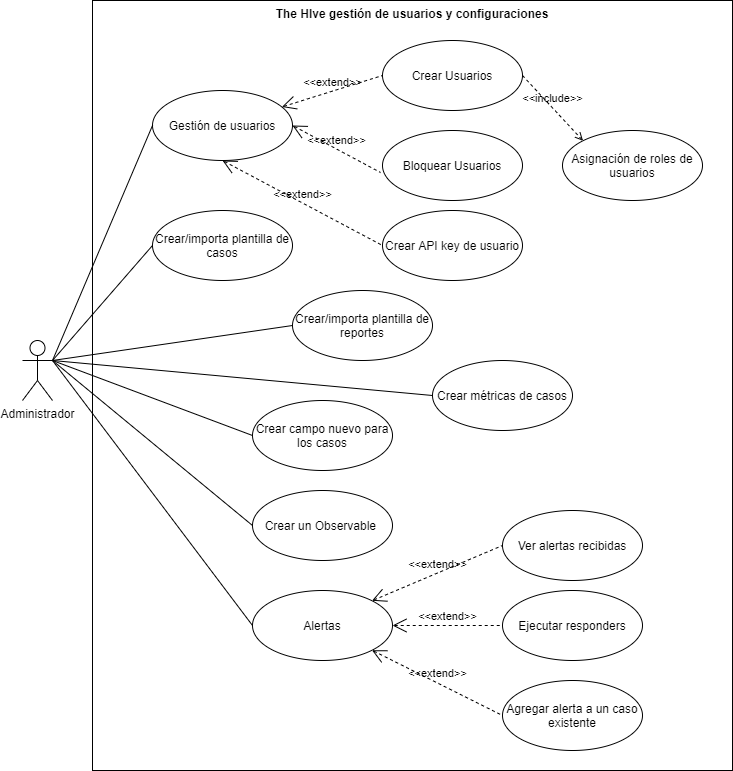
\includegraphics[width=1\textwidth]{./descripcion_sonion_imagenes/figura_28_thehive_user_conf.png}
        \caption{Casos de uso de gestión de usuario y configuraciones de TheHive}
        \label{fig:caso_de_uso_gestion_usuario_conf_thehive}
     \end{figure}
     \FloatBarrier
     En la figura \ref{fig:caso_de_uso_alertas_casos} se muestran las distintas opciones que se le presentan a un usuario de TheHive. Se aprecia que un usuario es capaz de visualizar alertas recibidas, agregar alertas a un caso existente y ejecutar responders de ser necesario. En cuanto a la gestión de casos, un usuario puede ver los casos existentes, crear uno nuevo, eliminar uno existente o unirlo con otro caso, cerrar un caso o en última instancia asignar este último a un usuario diferente. 
     \begin{figure}[H]
        \centering
        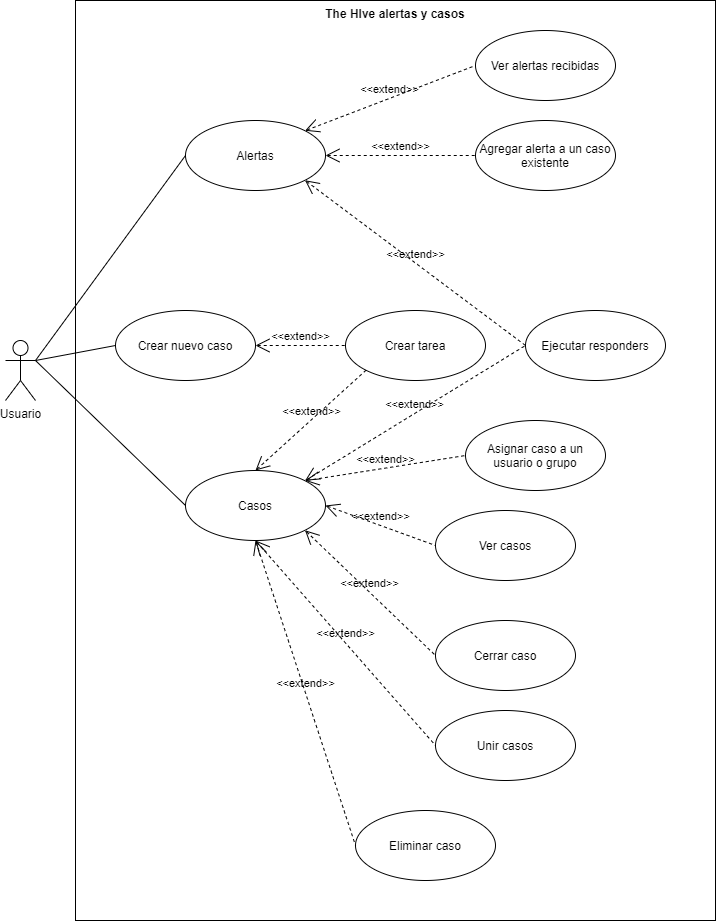
\includegraphics[width=1\textwidth]{./descripcion_sonion_imagenes/figura_29_thehive_alertas_casos.png}
        \caption{Diagrama de casos de uso de alertas y casos}
        \label{fig:caso_de_uso_alertas_casos}
     \end{figure}
     \pagebreak
     \begin{subsection}{Cortex}
        Luego de que el caso fue creado o sobre la misma alerta, el analista puede dar curso a una respuesta mediante “responders” que son scripts en los cuales se encuentra la respuesta del CSIRT a la amenaza. Tanto los responders como los analyzers se encuentran bajo la responsabilidad de Cortex, el subsistema encargado de procesar los casos de TheHive. Al final de esta sección, se presentan los diagramas de casos de uso correspondientes a Cortex.
        En la Figura \ref{fig:analizers_disponibles} se ven los analyzers disponibles. Estos son utilizados por los analistas para contrastar la información disponible con motores de búsqueda especializados como Shodan y VirusTotal. Los responders disponibles se observan en la Figura \ref{fig:ejemplos_responders_cortex}. Los analistas pueden activar o desactivar los mismos desde este panel.
     \begin{figure}[H]
        \centering
        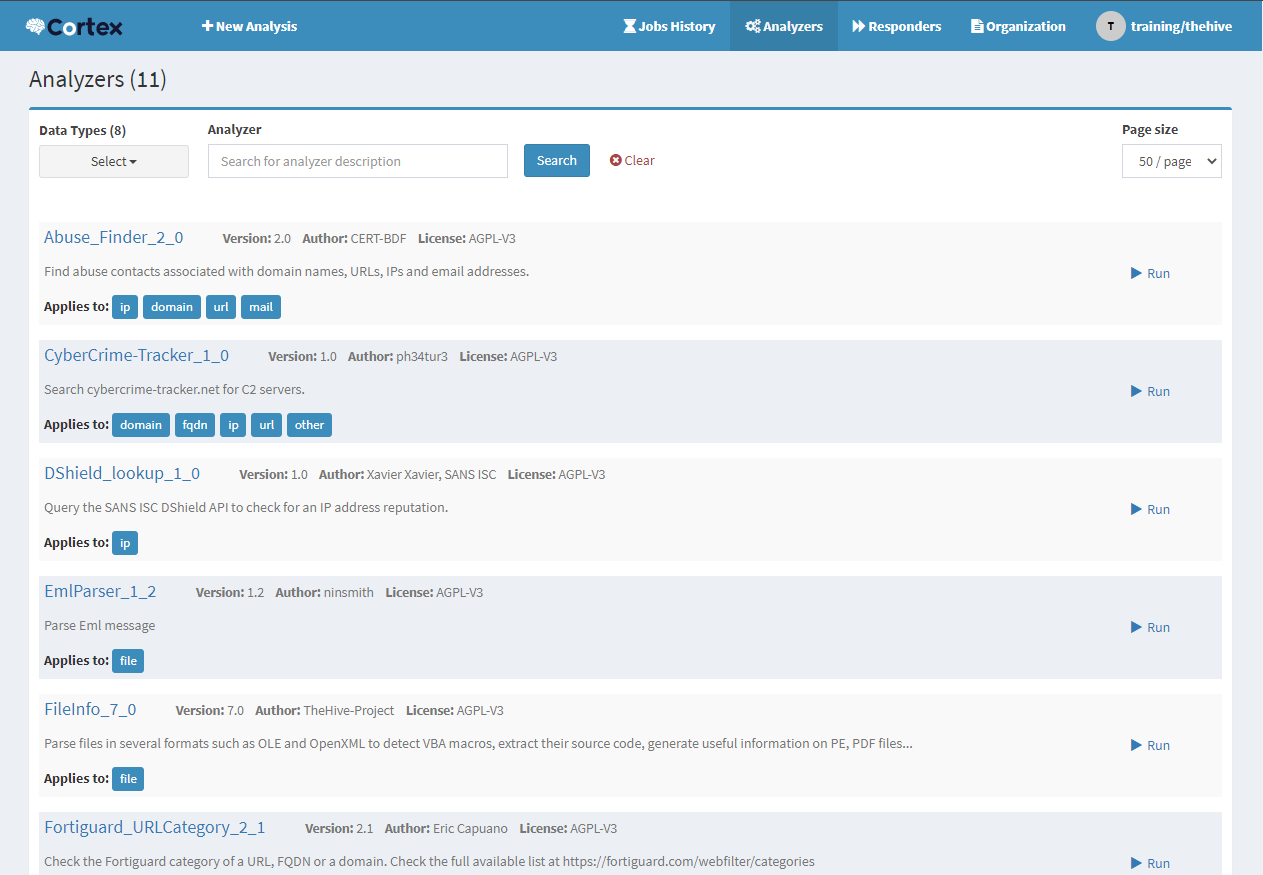
\includegraphics[width=1\textwidth]{./descripcion_sonion_imagenes/figura_26_analyzers_disponibles.png}
        \caption{Algunos de los analyzers disponibles en Cortex}
        \label{fig:analizers_disponibles}
     \end{figure}
     \begin{figure}[H]
        \centering
        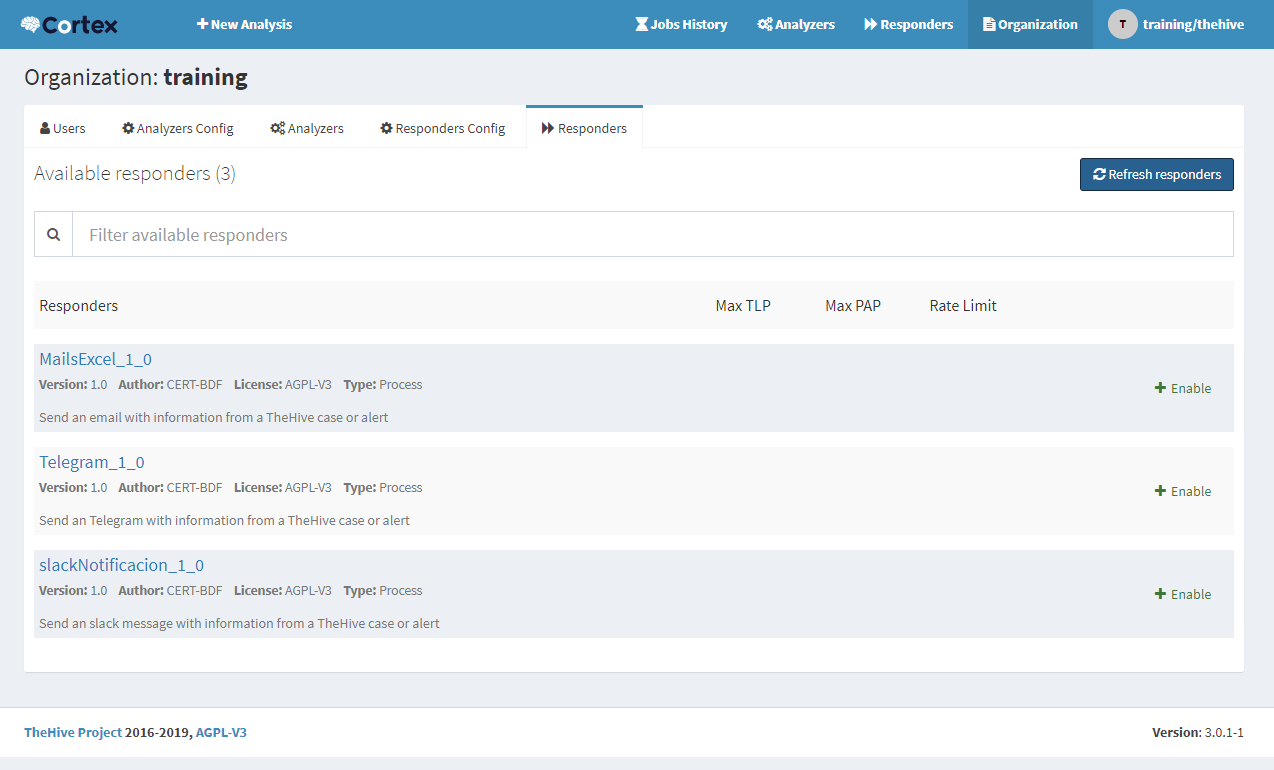
\includegraphics[width=1\textwidth]{./descripcion_sonion_imagenes/figura_27_responders_cortex.png}
        \caption{Ejemplos de responders utilizables en Cortex}
        \label{fig:ejemplos_responders_cortex}
     \end{figure}  
     \FloatBarrier
     En la Figura \ref{fig:caso_de_uso_gestion_usuarios_configuraciones_cortex} se observa el caso de uso de la gestion de usuarios y configuraciones para Cortex. Se muestran las capacidades de gestion tales como crear o bloquear usuarios, crear API KEYs para estos, crear organizaciones y agregarles usuarios a estas. Es posible asignar roles a los usuarios.
     %DIAGRAMA DE CASOS DE USOS DE CORTEX
     \begin{figure}[H]
        \centering
        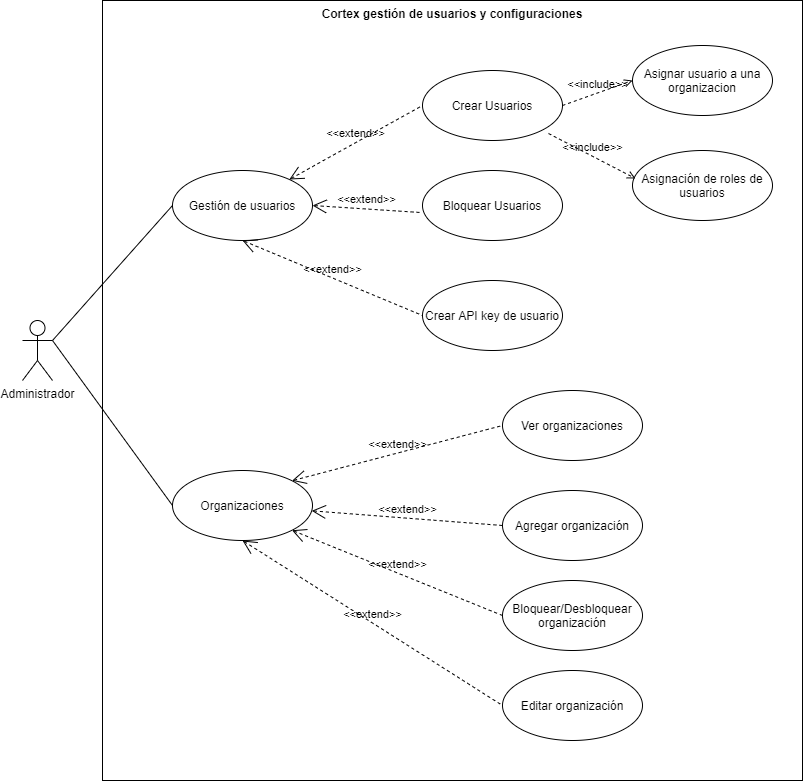
\includegraphics[width=1\textwidth]{./descripcion_sonion_imagenes/figura_30_cortex_user_conf.png}
        \caption{Casos de uso de gestión de usuario y configuraciones de Cortex}
        \label{fig:caso_de_uso_gestion_usuarios_configuraciones_cortex}
     \end{figure}
     \FloatBarrier
     En la Figura \ref{fig:caso_de_uso_tablero_cortex} se observa los casos de usos del panel de Cortex. Las primeras burbujas presentan las pestañas principales del menú de Cortex. El administrador puede crear usuarios de una organización, asignarles roles y permisos, configurar analyzers y responders para una organización.
     \begin{figure}[H]
      \centering
      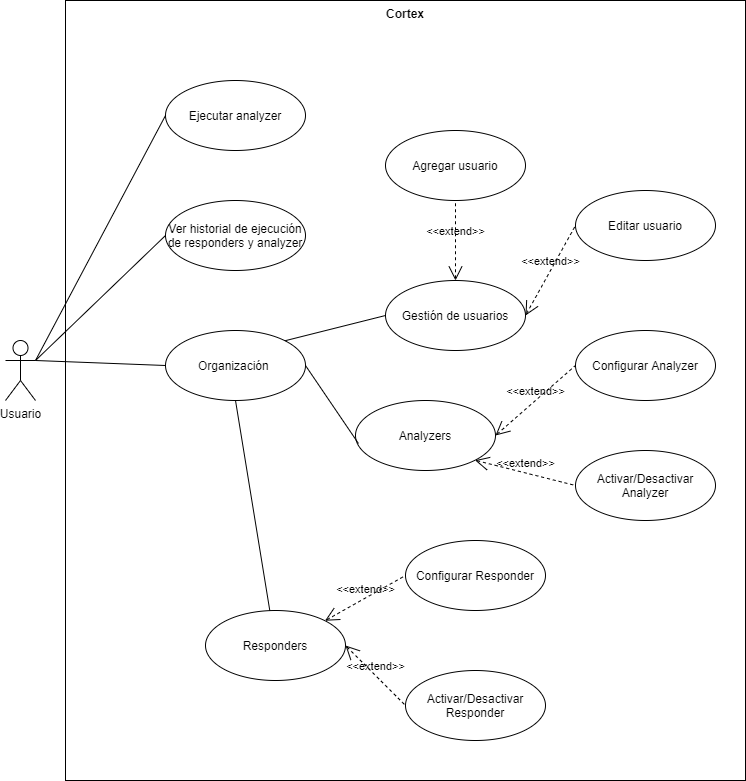
\includegraphics[width=1\textwidth]{./descripcion_sonion_imagenes/figura_31_cortex_tablero.png}
        \caption{Casos de uso del tablero de Cortex}
        \label{fig:caso_de_uso_tablero_cortex}
     \end{figure}
     \end{subsection}
   \end{section}

   \begin{section}{Integración con los sistemas de detección}
        En secciones anteriores se mencionó que Security Onion cuenta con NIDS y HIDS. Durante la configuración inicial del sistema se pueden especificar los NIDS a utilizar, para una configuración rápida de los sensores. Esto permite realizar una primera integración con el hardware disponible. Security Onion cuenta con OSSEC como HIDS para su autodefensa. La implementación de estos sistemas en el SIEM se llevo adelante en otro Proyecto Integrador.
   \end{section}
   \pagebreak
   \begin{subsection}{Suricata, Snort y Ossec}
        Suricata y Snort son motores de detección de amenazas en el tráfico de red. Ambos NIDS se basan en firmas o reglas para realizar la detección de amenazas. Estas firmas son actualizadas constantemente conforme a la aparición de nuevos tipos de ataques, exploits y malware. Si bien estos NIDS son gratuitos y de código abierto, Snort ofrece una versión paga, la cual cuenta con soporte para descargar las firmas actualizadas a la fecha. Por defecto Snort cuenta con las reglas básicas para la detección de amenazas bien conocidas. \par
    	Suricata, por otro lado, es desarrollado y mantenido por los colaboradores de la OISF, los cuales también dan soporte a las firmas ya que se actualizan las existentes y se agregan nuevas en forma permanente. Estas actualizaciones en las reglas son descargadas periódicamente mediante PulledPork, una utilidad que también es usada por Snort cuyo fin es descargar reglas y firmas desde distintos centros de investigación reconocidos en todo el mundo, como el SANS institute, Emerging Threats, entre otros. \par
        En el Cuadro \ref{table:4} se muestran las diferencias entre Snort y Suricata.
        \begin{table}[H]
            \centering
            \begin{tabular}{|m{10em}|m{11em}|m{11em}|}
                \hline 
               \multicolumn{1}{|c|}{Caracteristicas} & \multicolumn{1}{c|}{Snort} & \multicolumn{1}{c|}{Suricata}               \\ \hline % la primera fila se encuentra centrada
                    Desarrollador & CISCO & Open Information Security Foundation (OISF)  \\ 
                \hline
                    Lanzamiento  & 1998 & 2009 \\ 
                \hline
                    Lenguaje del código & C  & C  \\
                \hline
                    Sistema operativo & Linux, Windows y Mac OS X  & Linux, Windows y Mac OS X  \\
                \hline
                    Hilos & Monohilo  & Soporte múltiples hilos  \\
                \hline
                    Soporte IPv6 & Si  & Si  \\
                \hline
                    Reglas de Snort & Si  & Si \\
                \hline
                    Reglas de Emerging Threats & Si  & Si \\
                \hline
                    Formato de logs & unified2  & unified2   \\
                \hline
                    Compatible con Aanval & Si  & Si   \\
                \hline %linea final de tabla
            \end{tabular}
            \caption{Comparación entre Snort y Suricata}
            \label{table:4}
        \end{table}
        \FloatBarrier
        Por otro lado está OSSEC (reemplazado por  Wazuh en las versiones más recientes de Security Onion), es un IDS orientado a hosts (HIDS). Al igual que los NIDS anteriores está basado en firmas para la detección de amenazas, es gratuito y de código abierto. Las reglas pueden descargarse del repositorio disponible en github. \par
   \end{subsection}
   \begin{section}{Corolario del capítulo 4}
        En este capitulo se mostró la solución elegida, sus distintas arquitecturas, sus componentes internos y los subsistemas asociados. Se pudo apreciar a TheHive como una solución complementaria a Security Onion que contribuyo a mejorar la gestión de incidentes.
        En el capítulo siguiente se desarrollo la configuración de un ambiente de prueba y se desplegaron las soluciones mencionadas anteriormente en distintas topologías. Esto permitió dar cumplimiento a los requerimientos funcionales 1 y 3. \par
   \end{section}